\chapter{Projekt}
\section{Oprogramowanie PC}
\subsection{Struktura oprogramowania}
%>TODO czas przyszły, nie mów o ROSie i RViz jeszcze, to przyjdzie potem>wywal rviz i ros stad
%>TODO opisz procedurę połączenia oraz jego schemat

Robot wykonuje polecenia zadane przez aplikację sterującą oraz odpowiada na zapytania o dane. Aplikacja w ostatecznej wersji została zaimplementowana jako moduł platformy ROS\cite{ros} na systemie operacyjnym opartym o GNU/Linux. Po jej uruchomieniu ukazują się dwa okna - jedno jest oknem głównym do kontroli pojazdu, widoczne na Rys. \ref{fig:app-main-window}. Drugie to okno programu RViz w którym widoczny jest podgląd pozycji robota oraz mapy którą sporządza ukazane na Rys. \ref{fig:rviz-window}.

\subsubsection{Okno główne programu}
\begin{figure}[ht]
	\centering
		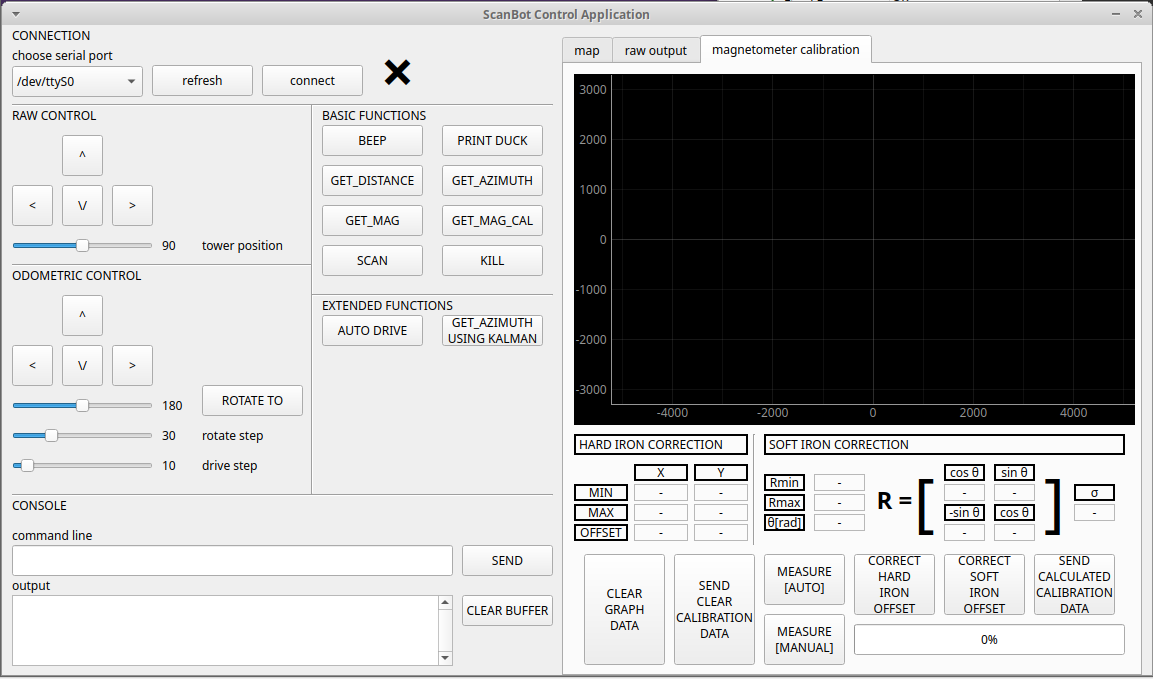
\includegraphics[width=1\linewidth]{rys/main-app-view-3.PNG}
	\caption{Okno główne aplikacji sterującej}
	\label{fig:app-main-window}
\end{figure}

Okno główne zostało podzielone na segmenty oraz zakładki w celu odseparowania poszczególnych funkcjonalności. Opis poszczególnych sekcji:

Sekcja \emph{CONNECTION} dotyczy połączenia portu szeregowego i zawiera elementy takie jak:
\begin{itemize}
    \item Lista rozwijana do wyboru portu szeregowego do którego wpięty jest konwerter USB-UART
    \item Przycisk \emph{refresh} odświeża listę
    \item Przycisk \emph{connect} inicjuje połączenie
    \item Ikona statusu połączenia - krzyżyk oznacza jego brak, zegarek oznacza oczekiwanie a symbol fajki oznacza zainicjowane połączenie
\end{itemize}

Sekcja \emph{RAW CONTROL} zawiera kontrolki sterujące robotem. Przytrzymanie każdego z przycisków odpowiada ruchowi robota w przód i w tył (kolejno strzałki w górę i w dół) lub obrotowi w lewo i w prawo (strzałki w lewo i w prawo). Po puszczeniu przycisku platforma zatrzymuje się bez zwłoki. Suwak służy do ustawiania pozycji wieżyczki pomiarowej, jest wyskalowany w stopniach.
\\

Sekcja \emph{ODOMETRIC CONTROL} służy do jazdy odometrycznej, tj. poruszając się za pomocą tych kontrolek uwzględniany jest przejechana trasa. Analogicznie jak w poprzedniej sekcji poruszanie kontrolowane jest przez strzałki, aczkolwiek tutaj nie należy ich przytrzymywać a jedynie krótko kliknąć. Po kliknięciu zostanie pokonany pewien dystans po którym robot się zatrzyma. Dystans do przejechania (krok) ustawiany jest za pomocą suwaka \emph{drive step} a wartość przez niego reprezentowana jest podana w centymetrach. Aby ustawić krok obrotu należy skorzystać z suwaka \emph{rotate step}. Przycisk \emph{ROTATE TO} służy do obracania robota na wyznaczony azymut, którego wartość wcześniej należy ustawić suwakiem znajdującym się obok niego. (Uwaga! Pojęcie azymutu w tym dokumencie oznacza kąt skierowania robota liczony od azymtu geograficznego 90°, przeciwnie do ruchu wskazówek zegara, czyli tak jak matematycznie reprezentowany jest kąt).
\\

Sekcja \emph{CONSOLE} pozwala na ręczne sterowanie robotem za pośrednictwem komend. Tutaj należy zaznaczyć że wszysktie funkcje sterujące oferowane przez program korzystają z tych komend odpowiednio je formułując i wysyłając do jednostki mobilnej. Pole tekstowe podpisane \emph{command line} służy do wprowadzania komendy, która jest wysyłana po kliknięciu przycisku \emph{SEND}.
Owa komenda pojawi się wtedy w polu tekstowym poniżej oznaczonym \emph{output}. Przycisk \emph{CLEAR BUFFER} wyczyści okno podglądu wraz z buforem nadawczym i odbiorczym, co przydaje się przy (na szczęście bardzo rzadkich) problemach z zerwaną komunikacją lub utratą synchronizacji sekwencji przesyłanych komend i odpowiedzi.
\\

Sekcja \emph{BASIC FUNCTIONS} posiada kolekcję przycisków wykonujących podstawowe funkcje robota niezwiązane z poruszaniem.
\begin{itemize}
    \item \emph{BEEP} powoduje wydanie 3 krótkich dźwięków przez robota
    \item \emph{PRINT DUCK} rysuje małą kaczkę na ekranie
    \item \emph{GET\_DISTANCE} mierzy i zwraca odległość od robota do przeszkody na którą aktualnie wycelowana jest wieżyczka
    \item \emph{GET\_AZIMUTH} mierzy i zwraca azymut w którym skierowany jest robot
    \item \emph{GET\_MAG} zwraca surowe dane z magnetometru (osie X i Y)
    \item \emph{GET\_MAG\_CAL} zwraca dane kalibracji magnetometru
    \item \emph{SCAN} skanuje otoczenie (obraca wieżyczkę i dokonuje serii 180 pomiarów odległości), po czym zwraca zmierzone wartości
    \item \emph{KILL} odłącza sygnał sterujący od serwomechanizmów
\end{itemize}

Sekcja \emph{EXTENDED FUNCTIONS} pozwala na wykonywanie bardziej złożonych zadań
\begin{itemize}
    \item \emph{AUTO DRIVE} załącza algorytm autonomiczej jazdy robota
    \item \emph{GET\_AZIMUTH USING KALMAN} wykonuje serię pomiarów i za pomocą prostej implementacji filtru Kalmana\cite{Kedzierski2016} zwraca przefiltrowany wynik reprezentujący azymut w którym robot jest skierowany
\end{itemize}

Zakładka \emph{map} (Rys. \ref{fig:main-app-map-section}) zawiera wykres który przedstawia mapę zmierzonych punktów. Przycisk \emph{CLEAR DATA} służy do czyszczenia całego wykresu.
\begin{figure}[ht]
	\centering
		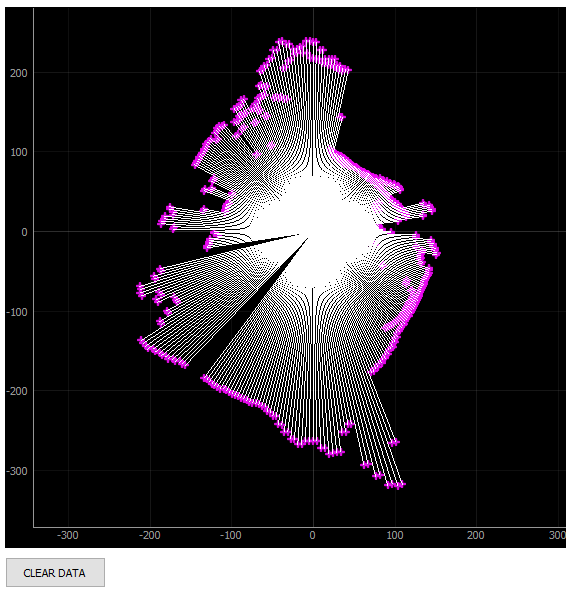
\includegraphics[width=0.8\linewidth]{rys/main-app-view-map.PNG}
	\caption{Zakładka \emph{map}}
	\label{fig:main-app-map-section}
\end{figure}

Zakładka \emph{raw output} (Rys. \ref{fig:main-app-raw-output-section}) zawiera pełnowymiarowy podgląd na historię wysyłanych i odbieranych danych. Jest większą wersją okienka \emph{output} sekcji \emph{CONSOLE}.
\begin{figure}[ht]
	\centering
		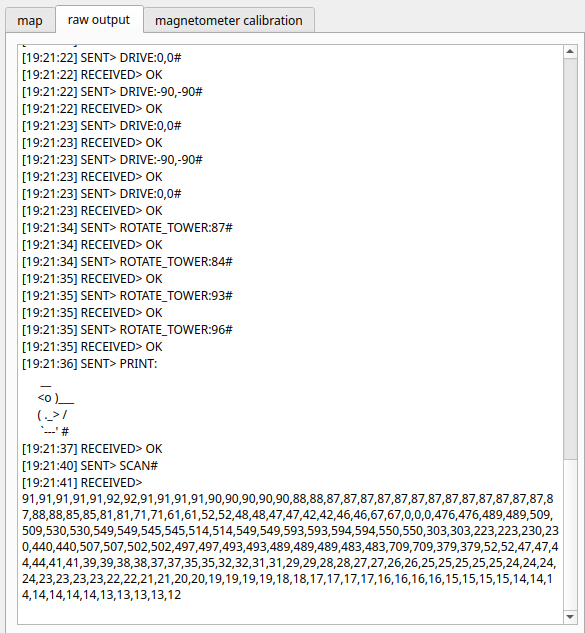
\includegraphics[width=0.8\linewidth]{rys/main-app-view-raw-output.PNG}
	\caption{Zakładka \emph{raw output}}
	\label{fig:main-app-raw-output-section}
\end{figure}

Zakładka \emph{magnetometer calibration} (Rys. \ref{fig:main-app-mag-section}) zawiera zestaw elementów wykorzystywanych do kalibracji magnetometru. Informacje o stosowanych metodach i przebiegu kalibracji znajdują się w rozdziale \ref{sec:odometry}.
\begin{figure}[ht]
	\centering
		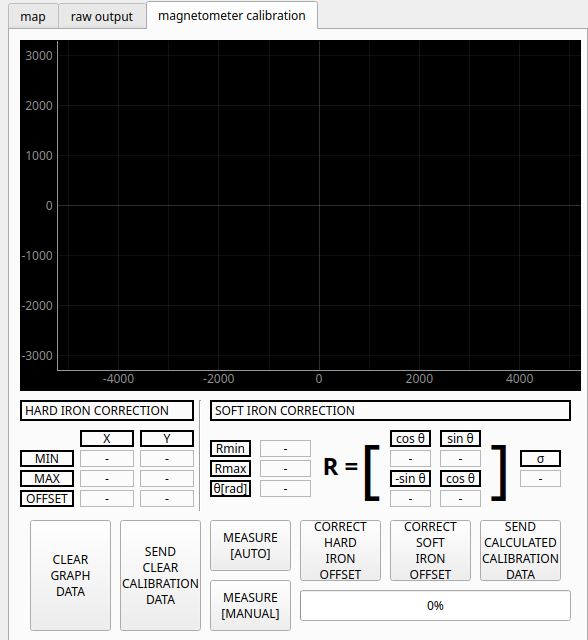
\includegraphics[width=0.8\linewidth]{rys/main-app-view-magnetom.PNG}
	\caption{Zakładka \emph{magnetometer calibration}}
	\label{fig:main-app-mag-section}
\end{figure}


\subsubsection{Program RViz}
\begin{figure}[ht]
	\centering
		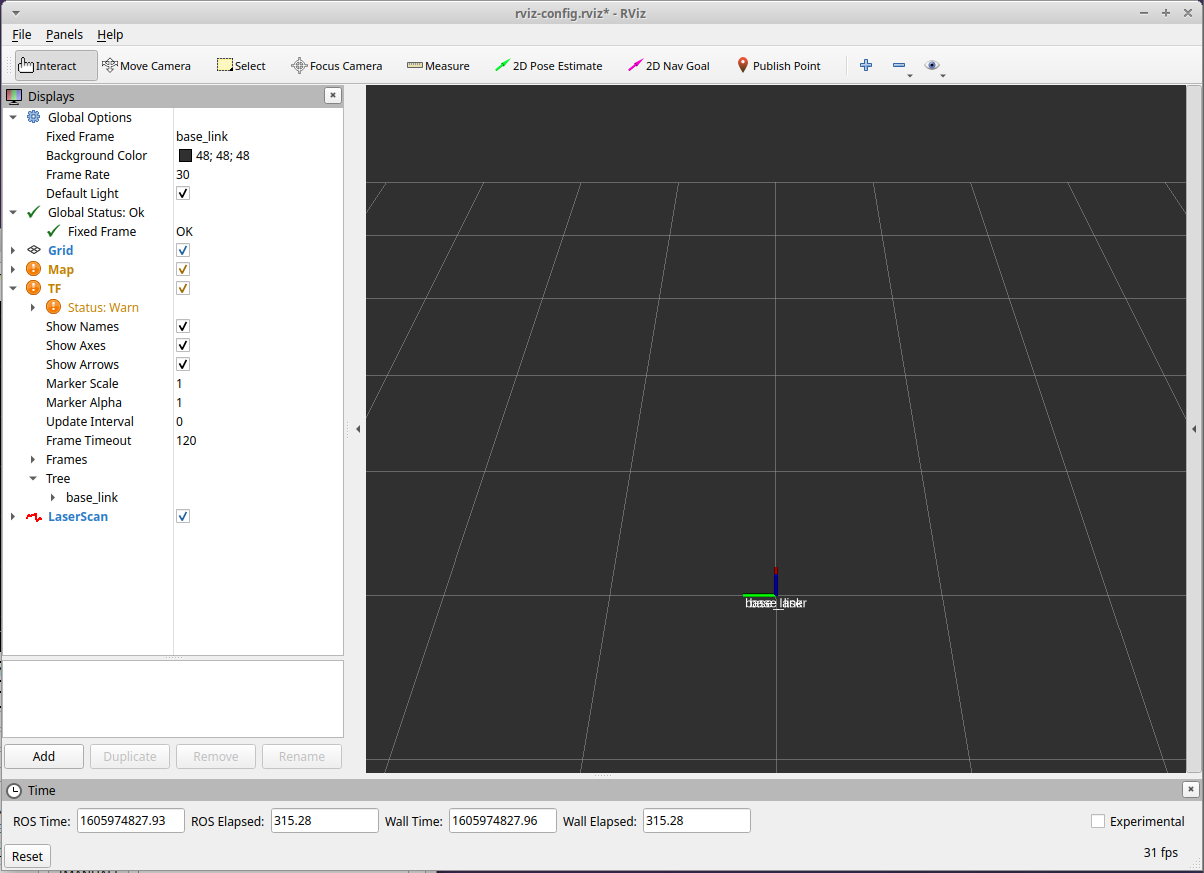
\includegraphics[width=1\linewidth]{rys/main-app-view-4.PNG}
	\caption{Okno programu RViz}
	\label{fig:rviz-window}
\end{figure}

Z okna głównego programu RViz należy zwrócić uwagę jedynie na podgląd układu współrzędnych po prawej stronie okna. Wszystkie parametry są ustawiane automatycznie wraz ze startem aplikacji, nie ma potrzeby żadnej ręcznej konfiguracji. Więcej informacji o tym programie dostępne jest na stronie internetowej \cite{rviz}.
Podczas pracy programu aktualna pozycja robota jest reprezentowana jako obiekt z etykietą \emph{base\_link} - podczas jazdy jego pozycja jest aktualizowana względem etykiety \emph{odom}. Na początku wszystkie układy współrzędnych są w pozycji zerowej i się nakładają.

\subsubsection{Środowisko sterujące}
\label{sec:ros-env}
\begin{figure}[ht]
	\centering
		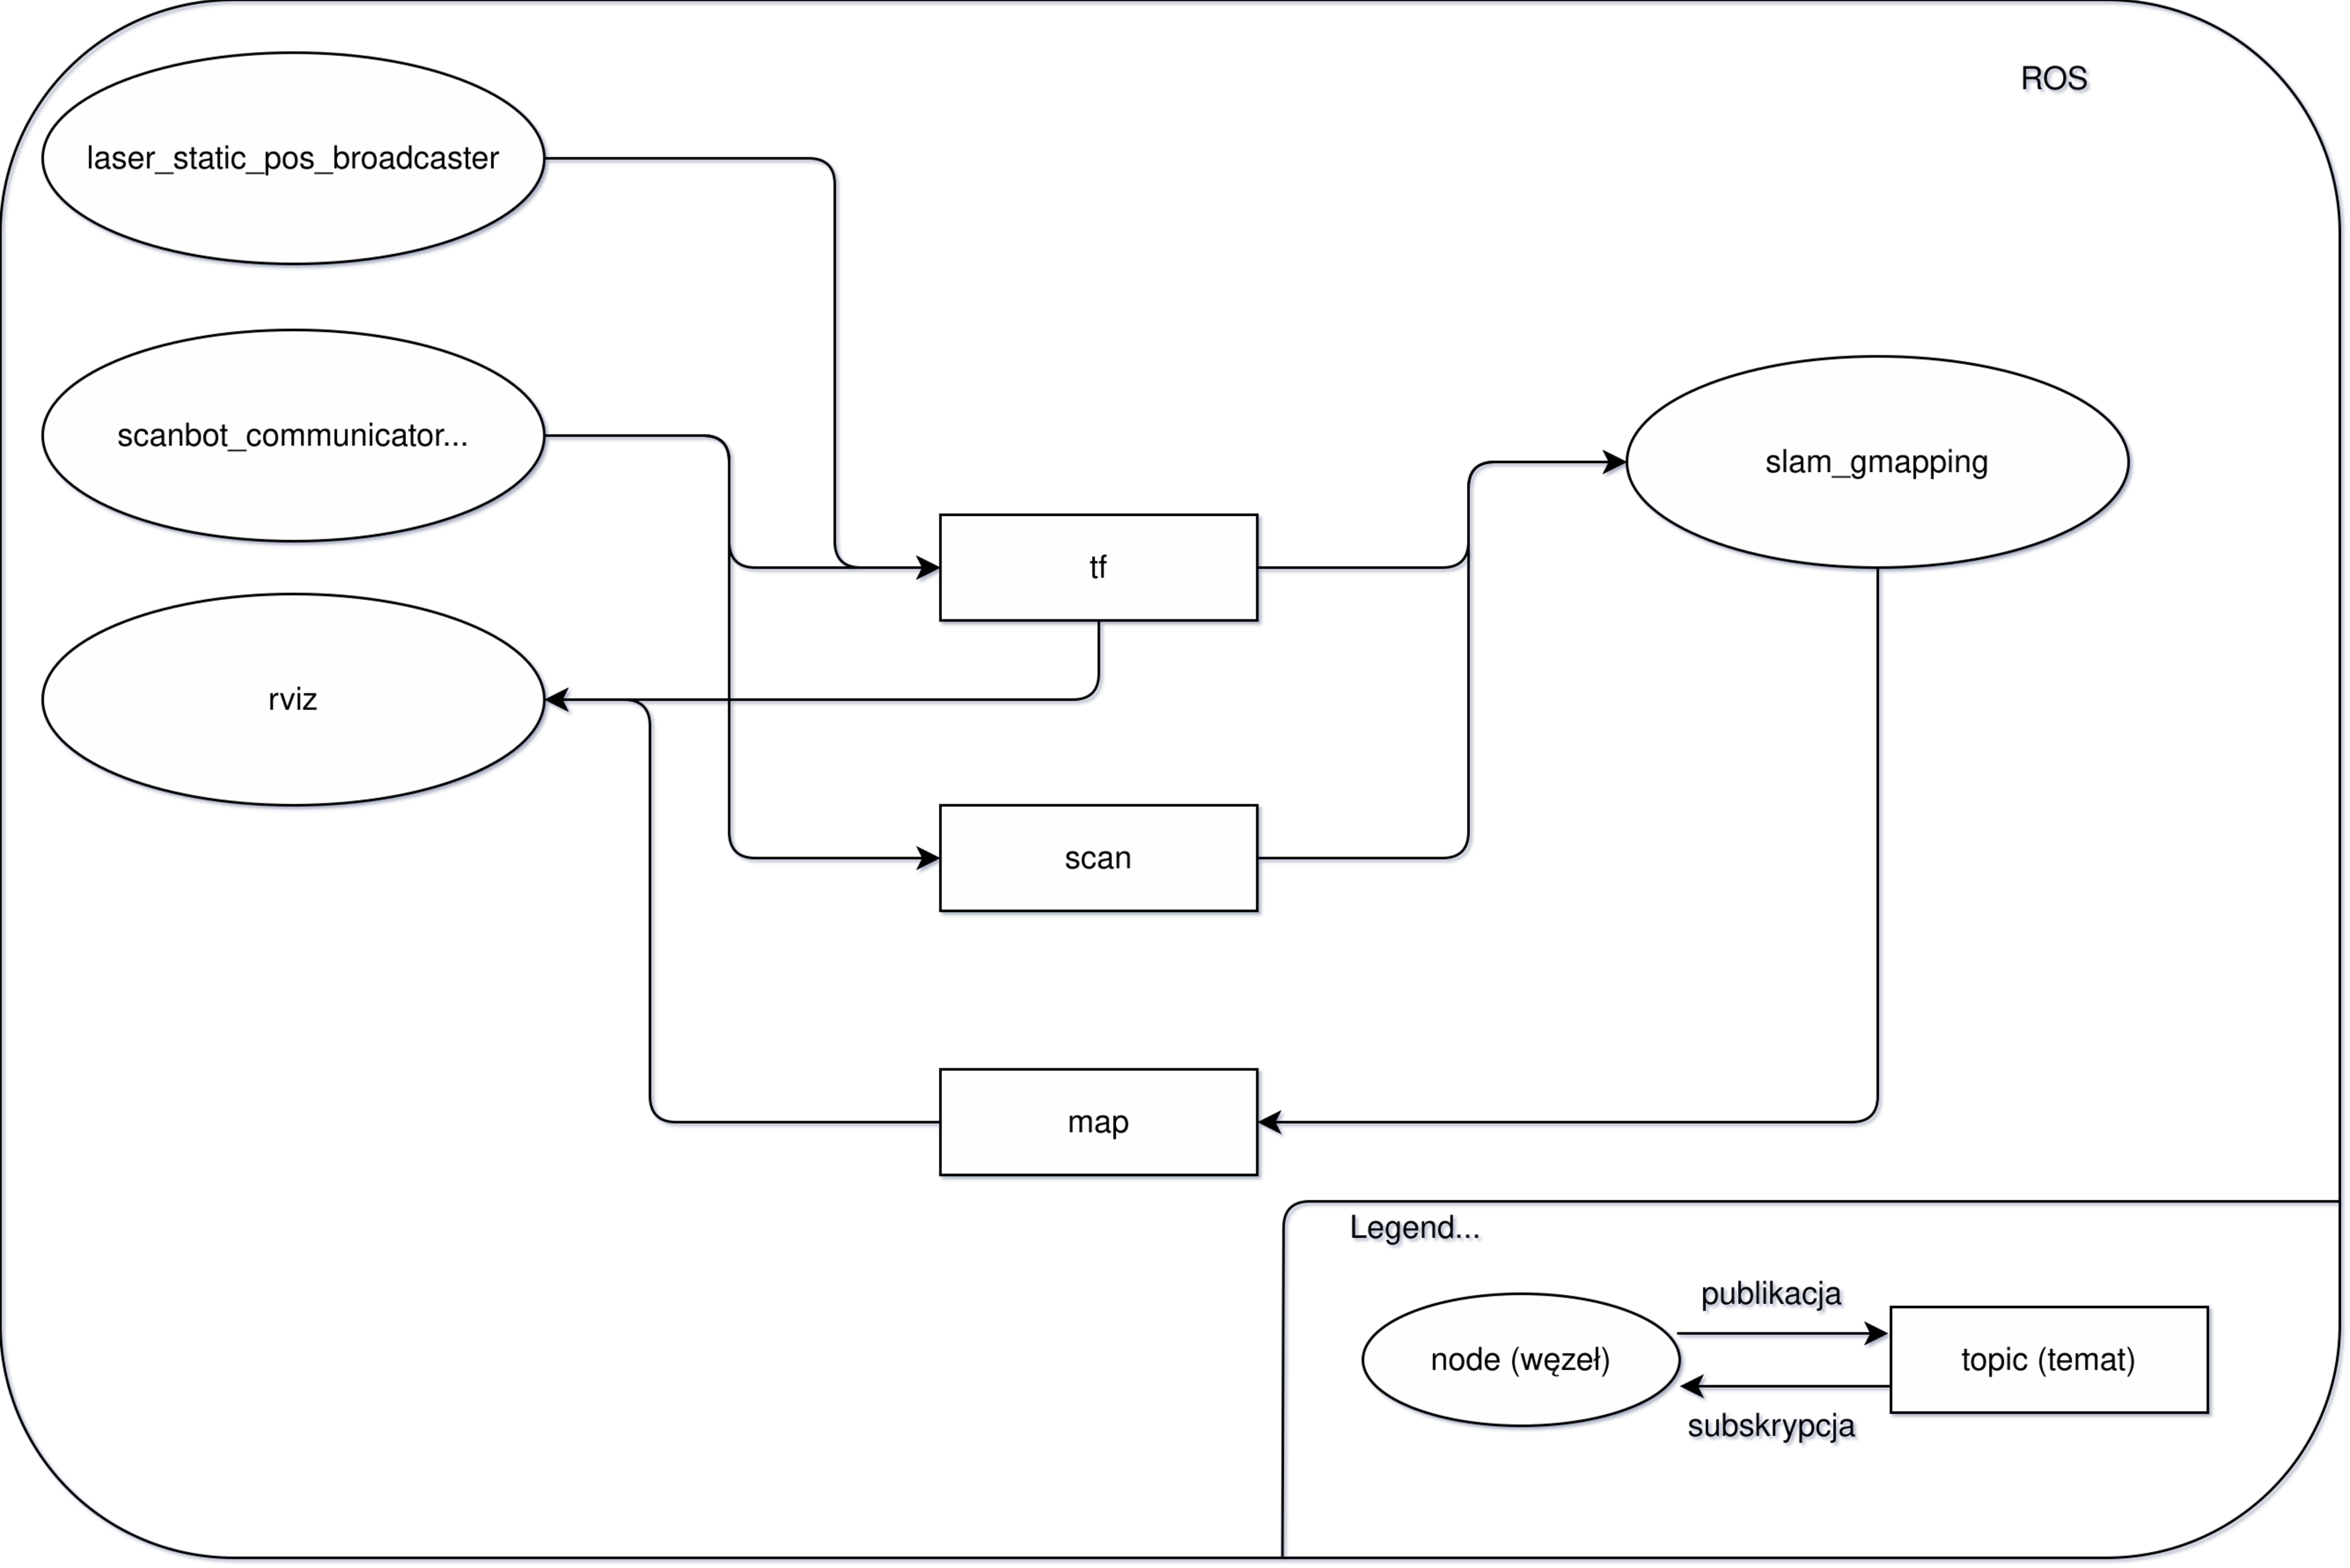
\includegraphics[width=1\linewidth]{rys/pc-application-infrastructure.pdf}
	\caption{Struktura środowiska ROS}
	\label{fig:pc-app-ros-infrastructure}
\end{figure}

Aplikacja komputerowa po uruchomieniu w środowisku ROS widoczna jest jako jeden z węzłów (node). W celu sporządzania mapy komunikuje się z innymi węzłami za pośrednictwem tematów (topics).
Na Rys. \ref{fig:pc-app-ros-infrastructure} ukazany jest schemat komunikacji poszczególnych węzłów.
Wykorzystywane są trzy tematy:
\begin{itemize}
    \item \emph{tf} jest tematem na którym publikowane są wszelkie translacje, czyli zależności między układami odniesienia
    \item \emph{scan} - tutaj publikowane są wyniki pomiarów odległości po wykonaniu skanu przez robota
    \item \emph{map} - na tym temacie pojawiają się dane reprezentujące mapę, wygenerowane przez algorytm \emph{gmapping}\cite{Grisetti2005}\cite{gmapping-website}\cite{gmapping-ros}
\end{itemize}

Ramki (frames), czyli w terminologii stosowanej w ROS układy odniesienia, a konkretnie ich względna pozycja są reprezentowane za pomocą wektorów zawierających dane o przesunięciu jak i obrocie. Więcej informacji na temat szczegółowego działania ramek można zasięgnąć na stronie internetowej ROS'a\cite{ros}. W niniejszym projekcie wykorzystywane są 4 ramki:
\begin{itemize}
    \item \emph{map} to główny układ odniesienia względem którego rysowana jest mapa
    \item \emph{odom} jest punktem odniesienia względem którego działa algorytm nawigacji zliczeniowej
    \item \emph{base\_link} odnosi się do bazy pojazdu, tj. środka względem którego się obraca podczas zakręcania
    \item \emph{base\_laser} to pozycja sensora skanującego
\end{itemize}
Wsyzstkie translacje między ramkami publikowane są na temacie \emph{tf}.

Węzeł \emph{laser\_static\_pod\_broadcaster} cyklicznie publikuje informację o położeniu modułu skanującego względem bazy robota. Jako że znajduje się ona bezpośrednio nad środkiem obrotu platformy, a sporządzana mapa jest dwuwymiarowa, jest to wektor zerowy.

Węzeł \emph{scanbot\_communicator} publikuje swoją pozycję na temacie \emph{tf} oraz podczas wykonywania skanu na kanale \emph{scan}.

Węzeł \emph{slam\_gmapping} subskrybuje kanały \emph{tf} i \emph{scan}. Na ich podstawie odpowiednio filtrując punkty uzyskane z pomiarów i dopasowując je do poprzednich algorytm tworzy mapę przeszkód widzianych przez robota.

Węzeł \emph{rviz} reprezentuje program RViz i subskrybuje dwa tematy - \emph{tf} oraz \emph{map}. Pozycje układów odniesienia reprezentowane są prze trójkolorowe trójwymiarowe obiekty, gdzie każdy z kolorów odpowiada jednej z osi (czerwony, zielony, niebieski odpowiadają kolejno osiom X, Y oraz Z). Ich położenie jest znane dzięki subskrypcji pierwszego z wymienionych tematów. Za pomocą danych przychodzących z drugiego z nich, program rysuje mapę pomieszczenia.


\subsubsection{Struktura aplikacji sterującej}
\begin{figure}[ht]
	\centering
		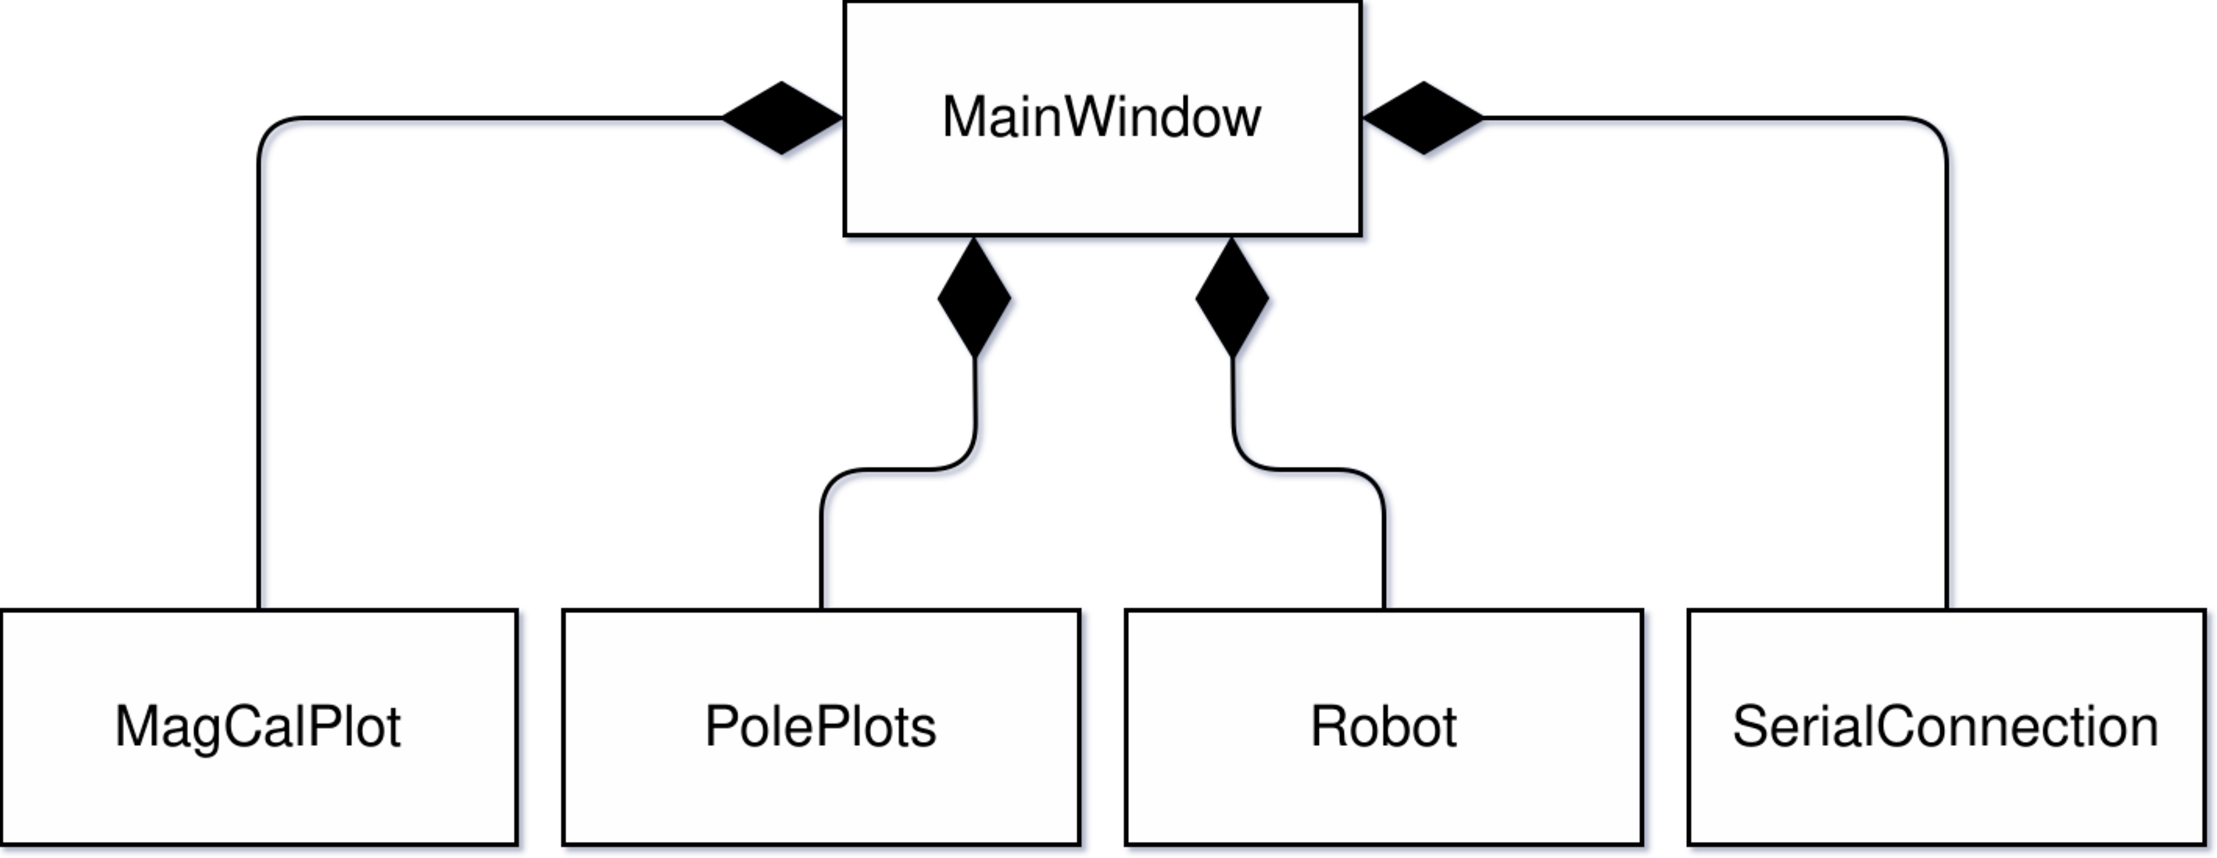
\includegraphics[width=0.8\linewidth]{rys/pc-application-simplified-uml.pdf}
	\caption{Uproszczony diagram kluczowych klas aplikacji}
	\label{fig:simple-class-diagram}
\end{figure}

W tej sekcji przedstawiony zostanie zarys najbardziej znaczących klas aplikacji sterującej. Jako że sama jej budowa nie jest kluczowym aspektem niniejszej pracy, dlatego po szczegółowe informacje dotyczące jej funkcjonowania autor odsyła do kodu źródłowego znajdującego się w dodatku A.

Na diagramie \ref{fig:simple-class-diagram} ukazano najważniejsze klasy głównego programu. Głównym obiektem jest tutaj okno, instancja klasy \emph{MainWindow}. Tutaj obsłużone jest kreowanie interfejsu graficznego, czyli ustawienie przycisków, pól tekstowych i innych elementów w odpowiednich miejscach, nadanie im identyfikatorów, ustawienie ciągów tekstowych, suwaków i innych elementów graficznych. Również akcje towarzyszące kliknięciom przycisków i przesuwaniu suwaków są tutaj przypisywane do odpowiednich funkcji. Funkcje te dla lepszej organizacji oraz czytelności zostały przeniesione do innych klas zorientowanych wokół konkretnych segmentów pracy aplikacji. Obiekty tych klas dostępne są poprzez zmienne wewnątrz głównej klasy.
\\

Klasa \emph{MagCalPlot} obsługuje szereg funkcji związanych z kalibracją magnetometru \ref{sec:mag_cal}. Zawiera przyciski uruchamiające funkcje związane z:
\begin{itemize}
    \item Czyszczeniem wykresu
    \item Rysowaniem zmierzonych danych w postaci punktów na wykresie
    \item Automatycznym pomiarem surowych danych z magnetometru
    \item Ręcznym pomiarem surowych danych z magnetometru
    \item Korekcją błędu \emph{hard iron} \cite{hard-iron} \cite{hard-soft-iron}
    \item Korekcją błędu \emph{soft iron} \cite{hard-soft-iron}
    \item Wysyłaniem danych kalibracyjnych do robota
\end{itemize}

Klasa \emph{PolePlots} obsługuje rysowanie punktów oraz czyszczenie wykresu zakładki \emph{map}. Przechowuje również dane o kolorach punktów jakie są na nim rysowane.

Klasa \emph{Robot} odzwierciedla surowy interfejs robota \label{sec:firmware}, dodając warstwę abstrakcji na surowe komendy wydawane mobilnej platformie i rozszerzając je - przykładowo podczas każdego z wywołanych funkcją pomiarów azymutu, jest on od razu publikowany na temacie \emph{tf}. Dodatkowo, w tej klasie obsłużony jest pomiar azymutu za pośrednictwem filtru Kalmana \cite{Kedzierski2016}. Również tutaj obsłużone jest publikowanie danych z odometrii i wykonywanych skanów na odpowiednich tematach, opisanych wcześniej w sekcji \ref{sec:ros-env} jak i również algorytm samodzielnej jazdy robota.

Klasa \emph{SerialConnection} służy do obsługi komunikacji interfejsu szeregowego konwertera USB-UART. Zawiera funkcje służące do nawiązywania połączenia, wysyłania komend i odbierania odpowiedzi od robota. Ponadto posiada uchwyt do klasy głównej, dzięki czemu wymieniane dane prezentuje zarówno w polu tekstowym w sekcji okna \emph{CONSOLE} jak i w zakładce \emph{raw output}.

\subsection{Jazda autonomiczna}
W celu realizacji samodzielnej jazdy robot został wyposażony w autorski algorytm pozwalający na omijanie napotkanych przeszkód i poruszanie się wzdłuż ścian. Operuje on na bardzo prostych zasadach - robot wykonuje kroki, pomiędzy którymi skanuje otoczenie i decyduje o podjętej akcji. Decyzja zapada na podstawie wykrycia przeszkód w wyznaczonych strefach. Ze względu na powiązanie z napisanym programem Rys. \ref{fig:autodrive-zones} przedstawia angielskie nazwy tychże stref. Ich kształt został wybrany ze względu na prostotę implementacji.
\begin{itemize}
    \item \emph{FRONT ZONE} (strefa F)
    \item \emph{LEFT ZONE 1} (strefa L1)
    \item \emph{LEFT ZONE 2} (strefa L2)
\end{itemize}

\begin{figure}[ht]
	\centering
		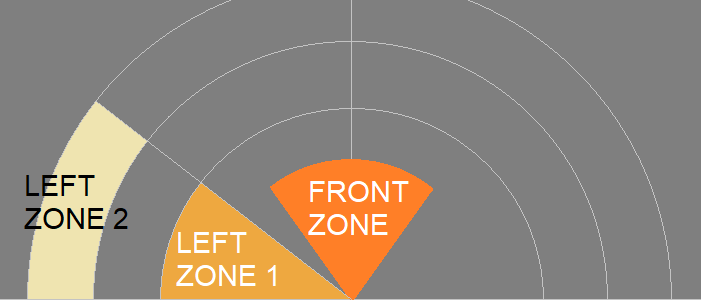
\includegraphics[width=1\linewidth]{rys/autodrive-zones.png}
	\caption{Strefy algorytmu jazdy autonomicznej}
	\label{fig:autodrive-zones}
\end{figure}

Należy zwrócić uwagę, że  Rys. \ref{fig:autodrive-zones} ma charakter poglądowy i nie jest wykonany w skali. Platforma znajduje się tutaj w punkcie środkowym układu współrzędnych, rysunek przedstawia zakres kątów od 0° do 180° , liczonych od kierunku prawego przeciwnie do ruchu wskazówek zegara. W tej samej kolejności przedstawiane są dane zeskanowane przez robota.
\\
Wymiary stref zostały dobrane metodą prób i błędów, dostrajane do momentu w którym robot był w stanie samodzielnie okrążyć pokój bez wjeżdżania w przeszkody.
Wielkości kroków to kolejne z parametrów którymi można regulować jakość pracy algorytmu. Rys. \ref{fig:autodrive-algorithm} prezentuje jego funkcjonowanie w oparciu o wymienione poniżej wartości.

\begin{itemize}
    \item zakres kątów obejmujących strefę \emph{F} to <70, 110>
    \item zakres kątów obejmujących strefy \emph{L1} i \emph{L2} to <140, 180>
    \item promień strefy \emph{F} wynosi 30 cm
    \item promień strefy \emph{L1} wynosi 50 cm
    \item strefa \emph{L2} jest wycinkiem zaczynającym się od promienia równego 70 cm, kończąca się na 90 cm
    \item mały krok jazdy do przodu wynosi 10 cm
    \item mały krok obrotu wynosi 10°
    \item duży krok obrotu wynosi 30°
\end{itemize}

\begin{figure}[ht]
	\centering
		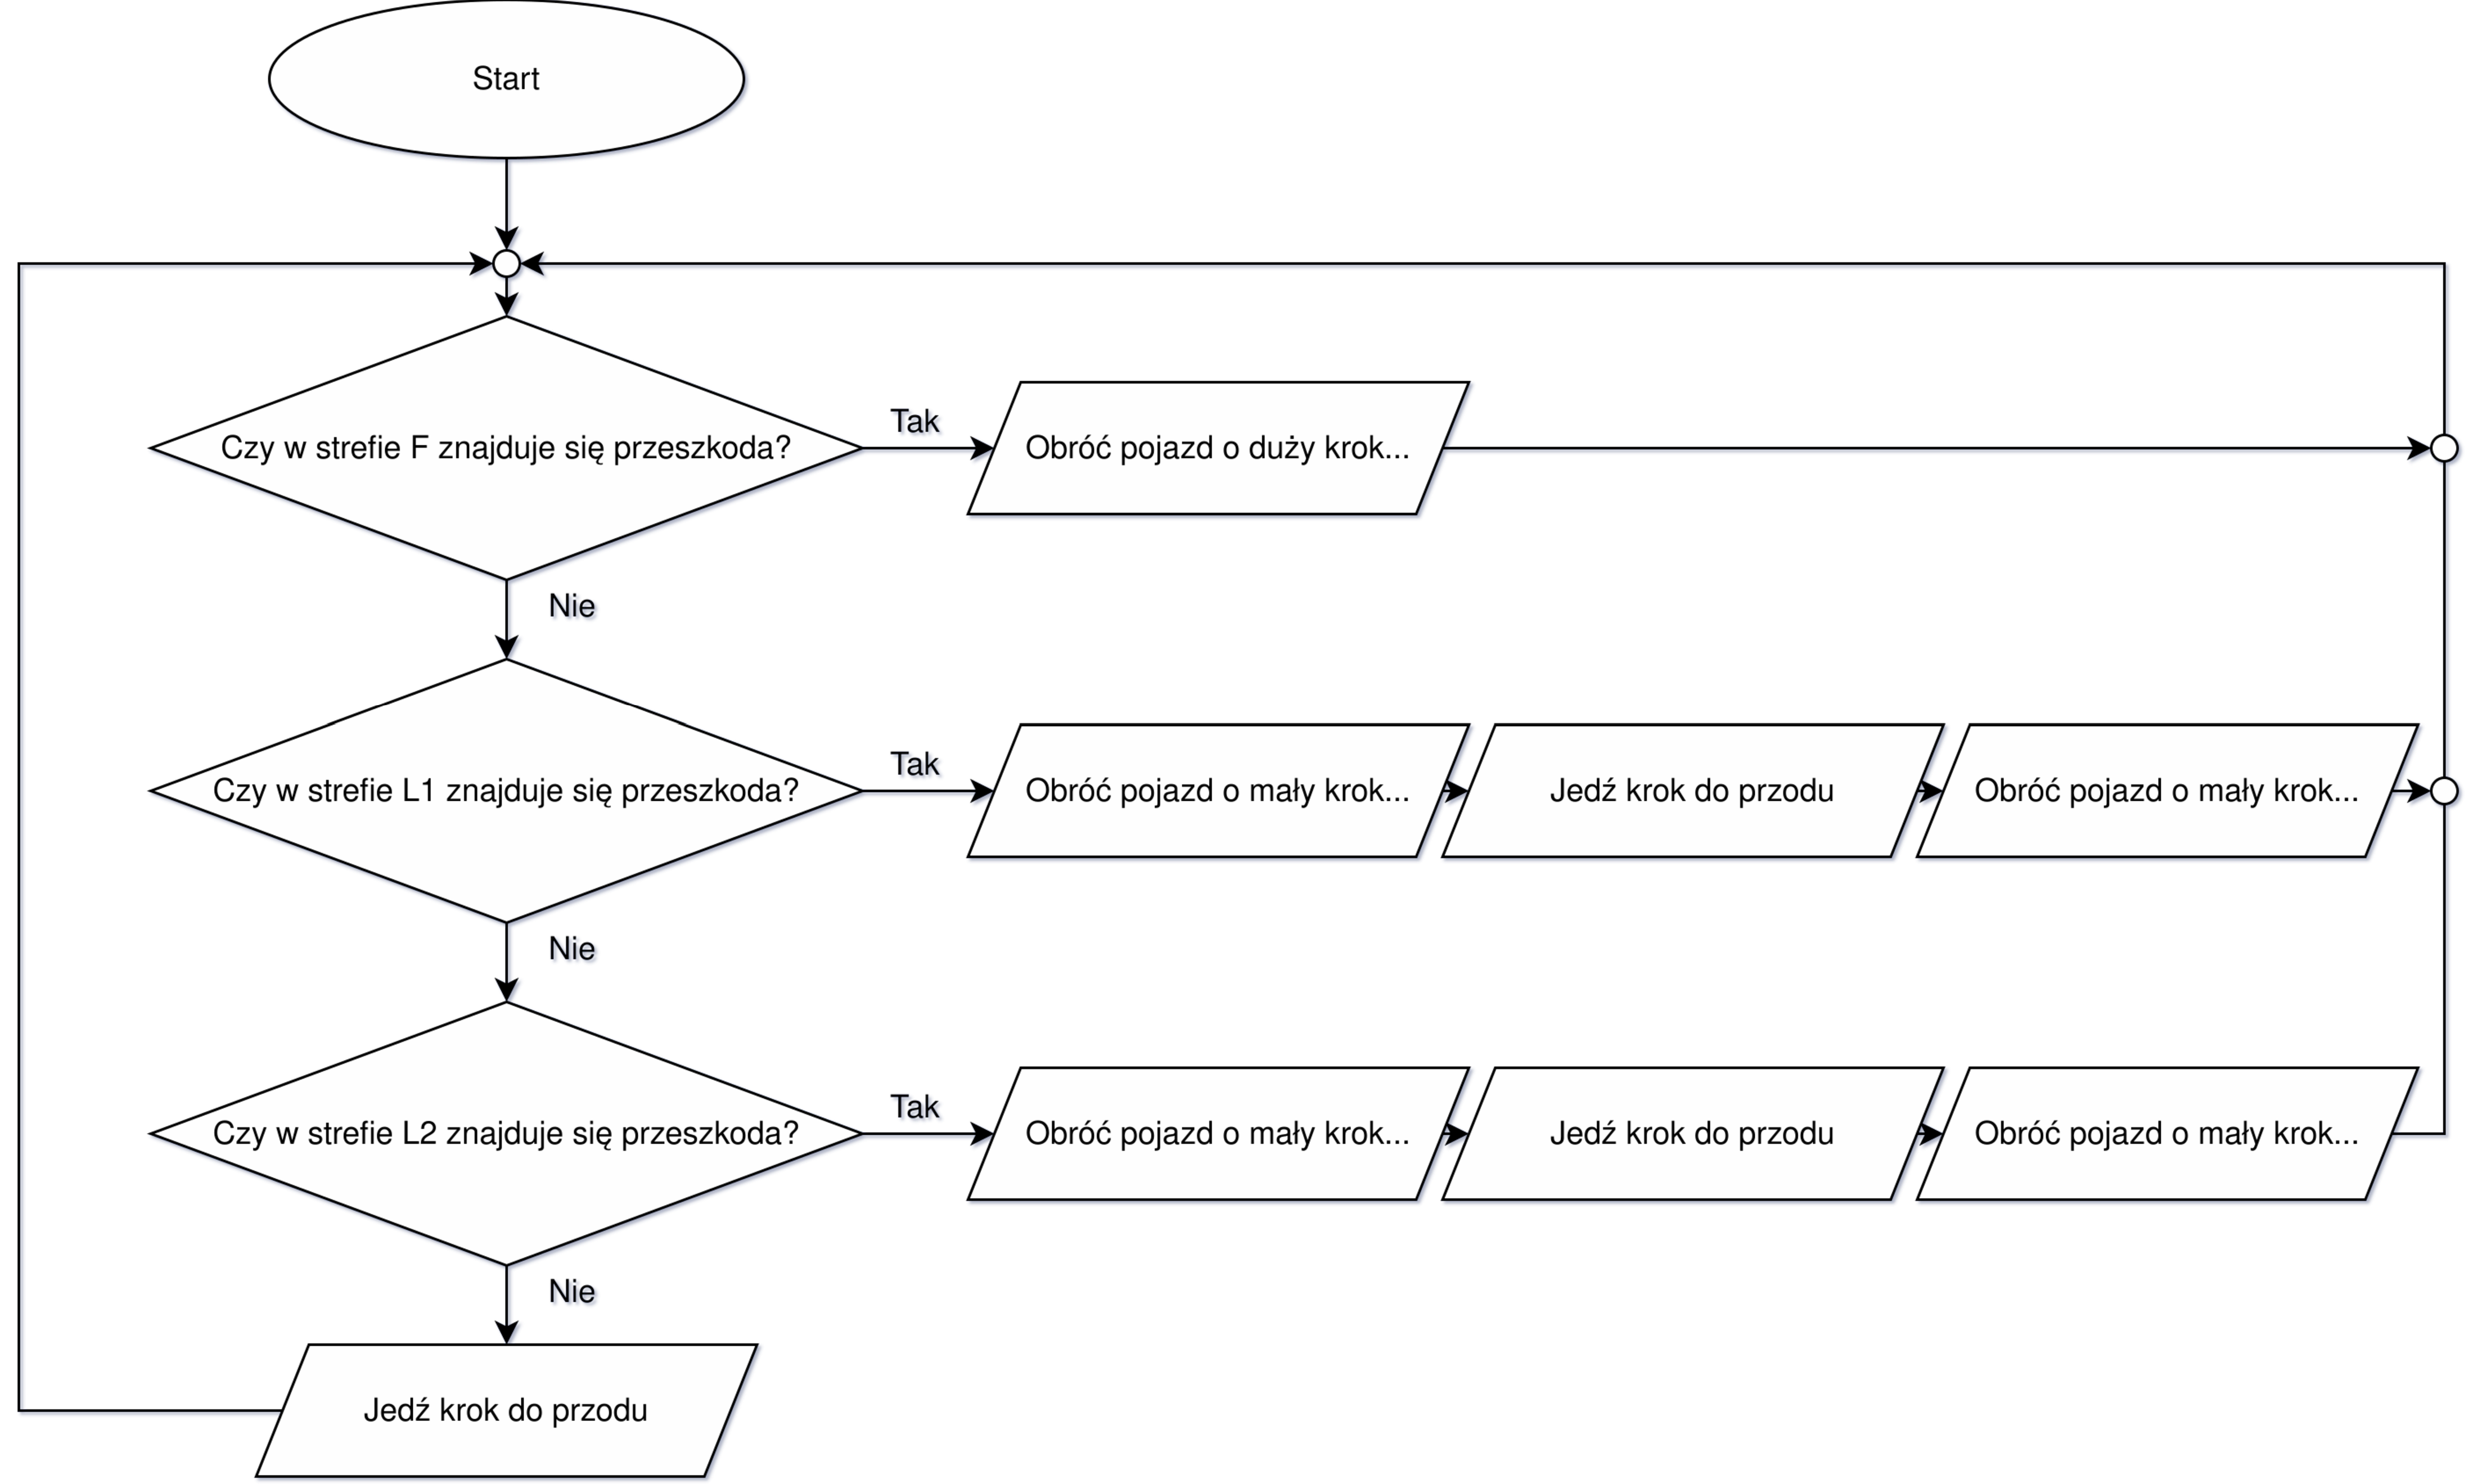
\includegraphics[width=1\linewidth]{rys/autodrive-algorithm.pdf}
	\caption{Algorytm jazdy autonomicznej}
	\label{fig:autodrive-algorithm}
\end{figure}

\section{Firmware}
\label{sec:firmware}
Dzięki zastosowaniu mikrokontrolera jako jednostki sterującej mobilną platformą skanującą zużycie prądu jest bardzo małe (bez peryferiów zużywa <51mA\cite{stm32-datasheet}). Nakłada to niestety ograniczenia związane z mocą obliczeniową urządzenia i dostępną pamięcią w której przechowywany jest program. 

Pierwszym kierunkiem w którym udał się autor były popularne dziś płytki Arduino, czego głównym powodem jest łatwość szybkiego prototypowania i szeroki wachlarz gotowych rozwiązań obsługujących różne sensory, serwomechanizmy, wyświetlacze i wiele innych. Płytka nie powinna być zbyt duża, dlatego na uwadze były mniejsze egzemplarze takie jak np. Arduino Nano. Jednak ze względu na niskie taktowanie procesora (16MHz) i niewiele pamięci Flash (32kB) na program wybrana została alternatywa - tzw. płytka ``blue pill``\cite{bluepill}. Jest to nieoficjalna płytka, podobna do Arduino. Można ją zaś programować w tym samym środowisku i wykorzystywać wiele (choć nie wszystkie) z bibliotek napisanych pod oficjalnie wspierane płytki. Jest tak dzięki zestawowi bibliotek STM32duino \cite{stm32duino-github} zapewniających kompatybilność z wcześniej wspomnianym środowiskiem. Do kompilacji i wgrania programu zostało wykorzystane kompatybilne z Arduino - PlatformIO IDE \cite{platformio}.
\\

Program działający na platformie wykonuje jedynie proste polecenia odebrane od aplikacji sterującej i odpowiada prostym potwierdzeniem, wartością lub listą wartości. Poniżej wylistowano polecenia:

\begin{enumerate}
    \item \emph{DRIVE} - ustaw zadaną prędkość na gąsienicach
    \item \emph{ROTATE\_TOWER} - obróć wieżyczkę na żądaną pozycję
    \item \emph{KILL} - odłącz sygnał sterujący od serwomechanizmów
    \item \emph{PRINT} - pokaż tekst na wyświetlaczu
    \item \emph{BEEP} - wydaj serię dźwięków o zdefiniowanej liczbie i czasie trwania
    \item \emph{GET\_MAG} - zwróć surowy pomiar z osi X i Y magnetometru
    \item \emph{GET\_AZIMUTH} - zwróc azymut w którym skierowany jest robot
    \item \emph{GET\_DISTANCE} - zmierz odległość od przeszkody
    \item \emph{GET\_TIME} - zwróć wartość czasu w milisekundach od uruchomienia robota
    \item \emph{MOVE} - przemieść się o zadany dystans do przodu lub do tyłu
    \item \emph{ROTATE\_TO} - obróć się na zadany azymut
    \item \emph{ROTATE} - obróć się o kąt
    \item \emph{SCAN} - skanuj otoczenie
    \item \emph{SET\_MAG\_CAL} - ustaw wartości do kalibracji magnetometru
    \item \emph{GET\_MAG\_CAL} - pobierz wartości kalibracji
    \item \emph{RESET} - uruchom ponownie robota
\end{enumerate}

>TODO wyjaśnić parametry komend

\section{Schemat budowy mechanicznej}
Główną przeszkodą w nawigacji zliczeniowej jest kumulujący się błąd. Wynika on z czynników niemożliwych do zwalczenia w całości, które są naturalne w każdym fizycznym obiekcie. Do tych czynników można zaliczyć: 
\begin{enumerate}
    \item poślizg kół pojazdu
    \item bezwładność - brak możliwości niezwłocznego zatrzymania pojazdu w punkcie
    \item niedokładność urządzeń pomiarowych wynikającą z ich fizycznych właściwości, m. in. szumów i zakłóceń
\end{enumerate}

Do pierwszych dwóch wymienionych czynników bezpośrednio odwołuje się jedna z decyzji projektowych. W pojeździe zostanie zastosowany gąsienicowy układ bieżny. Zwiększenie powierzchni kontaktu z podłogą zapewni bardziej stabilny obrót i jazdę platformy. Pomoże również w szybszym jej zatrzymaniu. Do trzeciego punktu sam projekt mechaniczny nie ma żadnego odniesienia, ta kwestia zostanie omówiona w podrozdziale \ref{sec:kalman}.

Projekt został wykonany w programie Autodesk Inventor \cite{inventor}. Pliki projektu są dostępne w dodatku A \label{sec:disc-addon}. Rzuty projektu przedstawione są na rysunkach \ref{fig:view1}, \ref{fig:view2} i \ref{fig:view3}. Robot powstanie na drukarce 3D działającej w technologii FDM (ang. \emph{Fused Deposition Modeling}) z materiału PLA (ang. PolyLactic Acid).

>TODO powiedzieć o przeniesieniu napędu, enkoderach, przełożeniu
>TODO powiedzieć o celu montowania wyświetlacza, przycisku wł. wył., sposobie ładowania i nacięciu wykonywanym z tyłu na przewody.


\begin{figure}[H]
	\centering
		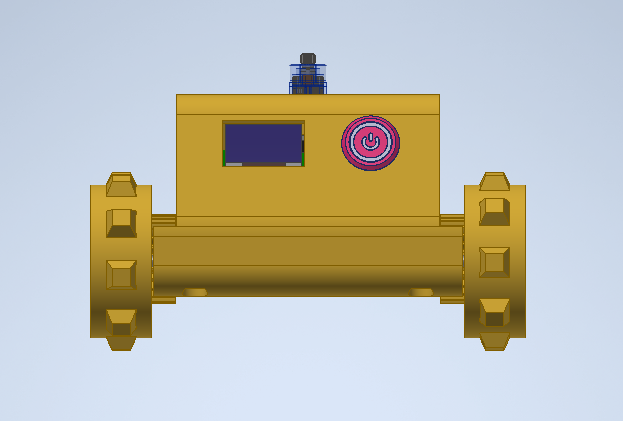
\includegraphics[width=0.5\linewidth]{rys/view1.png}
	\caption{Rzut główny platformy}
	\label{fig:view1}
\end{figure}

\begin{figure}[H]
	\centering
		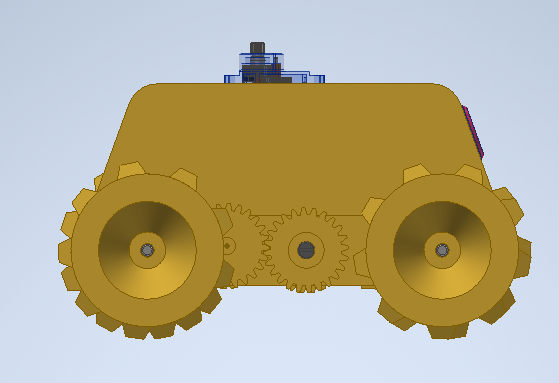
\includegraphics[width=0.5\linewidth]{rys/view2.png}
	\caption{Rzut platformy z prawej strony}
	\label{fig:view2}
\end{figure}

\begin{figure}[H]
	\centering
		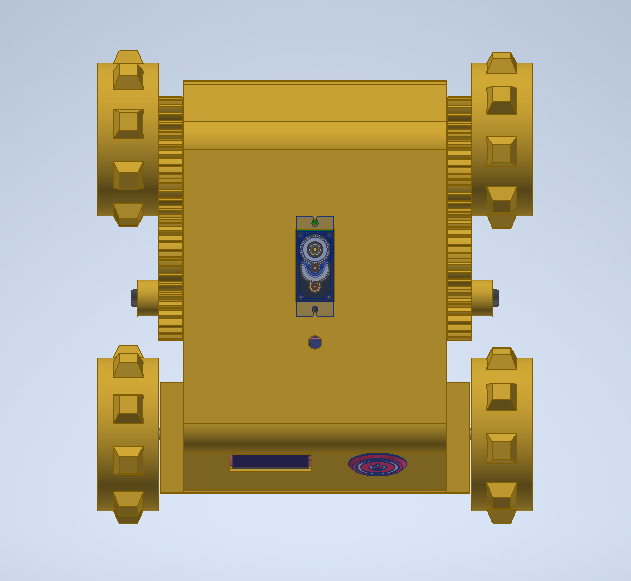
\includegraphics[width=0.5\linewidth]{rys/view3.png}
	\caption{Rzut platformy z góry}
	\label{fig:view3}
\end{figure}

Wieżyczka przedstawiona w rzucie izometrycznym na Rys. \ref{fig:tower} została zaprojektowana osobno. Sensor zostanie zamontowany w przesunięciu względem osi w celu częściowej redukcji jego martwej strefy. Powstanie w ten sam sposób i z tego samego materiału co reszta platformy.

\begin{figure}[ht]
	\centering
		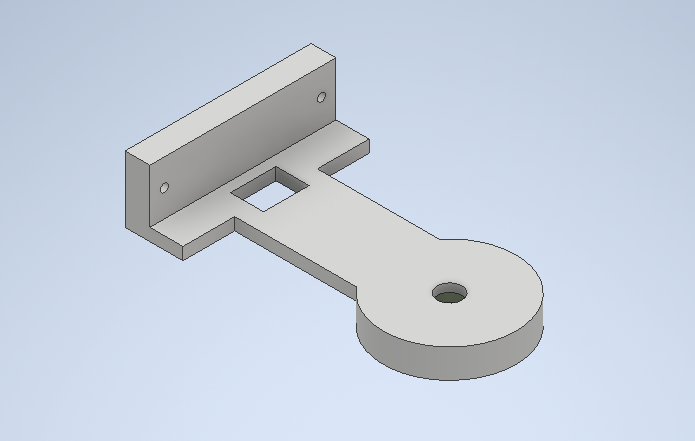
\includegraphics[width=0.5\linewidth]{rys/arm.png}
	\caption{Rzut izometryczny wieżyczki}
	\label{fig:tower}
\end{figure}

Gąsienica widoczna na Rys. \ref{fig:tracks} będzie wydrukowana w innym materiale - elastycznym TPU (ang. \emph{Thermoplastic PolyUrethane}). Potrzebne będą dwa egzemplarze - po jednym na stronę. Aby zniwelować poślizg względem kół a także przenieść napęd z tylnych na przednie, jej projekt posiada otwory wpasowujące się w wypustki na kołach. Dla redukcji poślizgu względem miękkich podłoży sama posiada wypustki na powierzchni zewnętrznej.

\begin{figure}[ht]
	\centering
		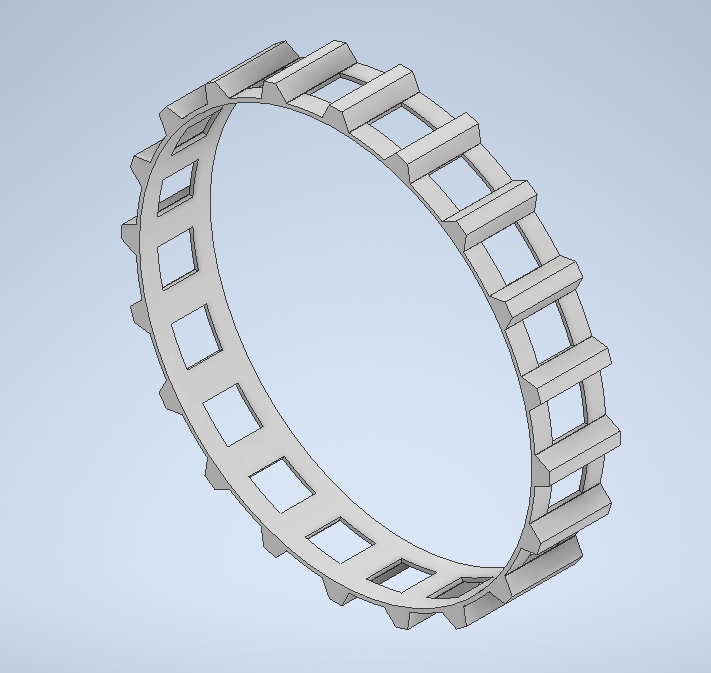
\includegraphics[width=0.5\linewidth]{rys/tracks-final.png}
	\caption{Rzut izometryczny gąsienicy}
	\label{fig:tracks}
\end{figure}



\section{Schemat elektroniczny}
>TODO napisac czemu bluetooth, czemu laser i czemu wszystkie inne elementy zostały wybrane
>TODO dac cite do linkow produktow, omowic kazdy wykorzystany
>TODO moze zrob dokladniejszy schemat

\begin{figure}[ht]
	\centering
		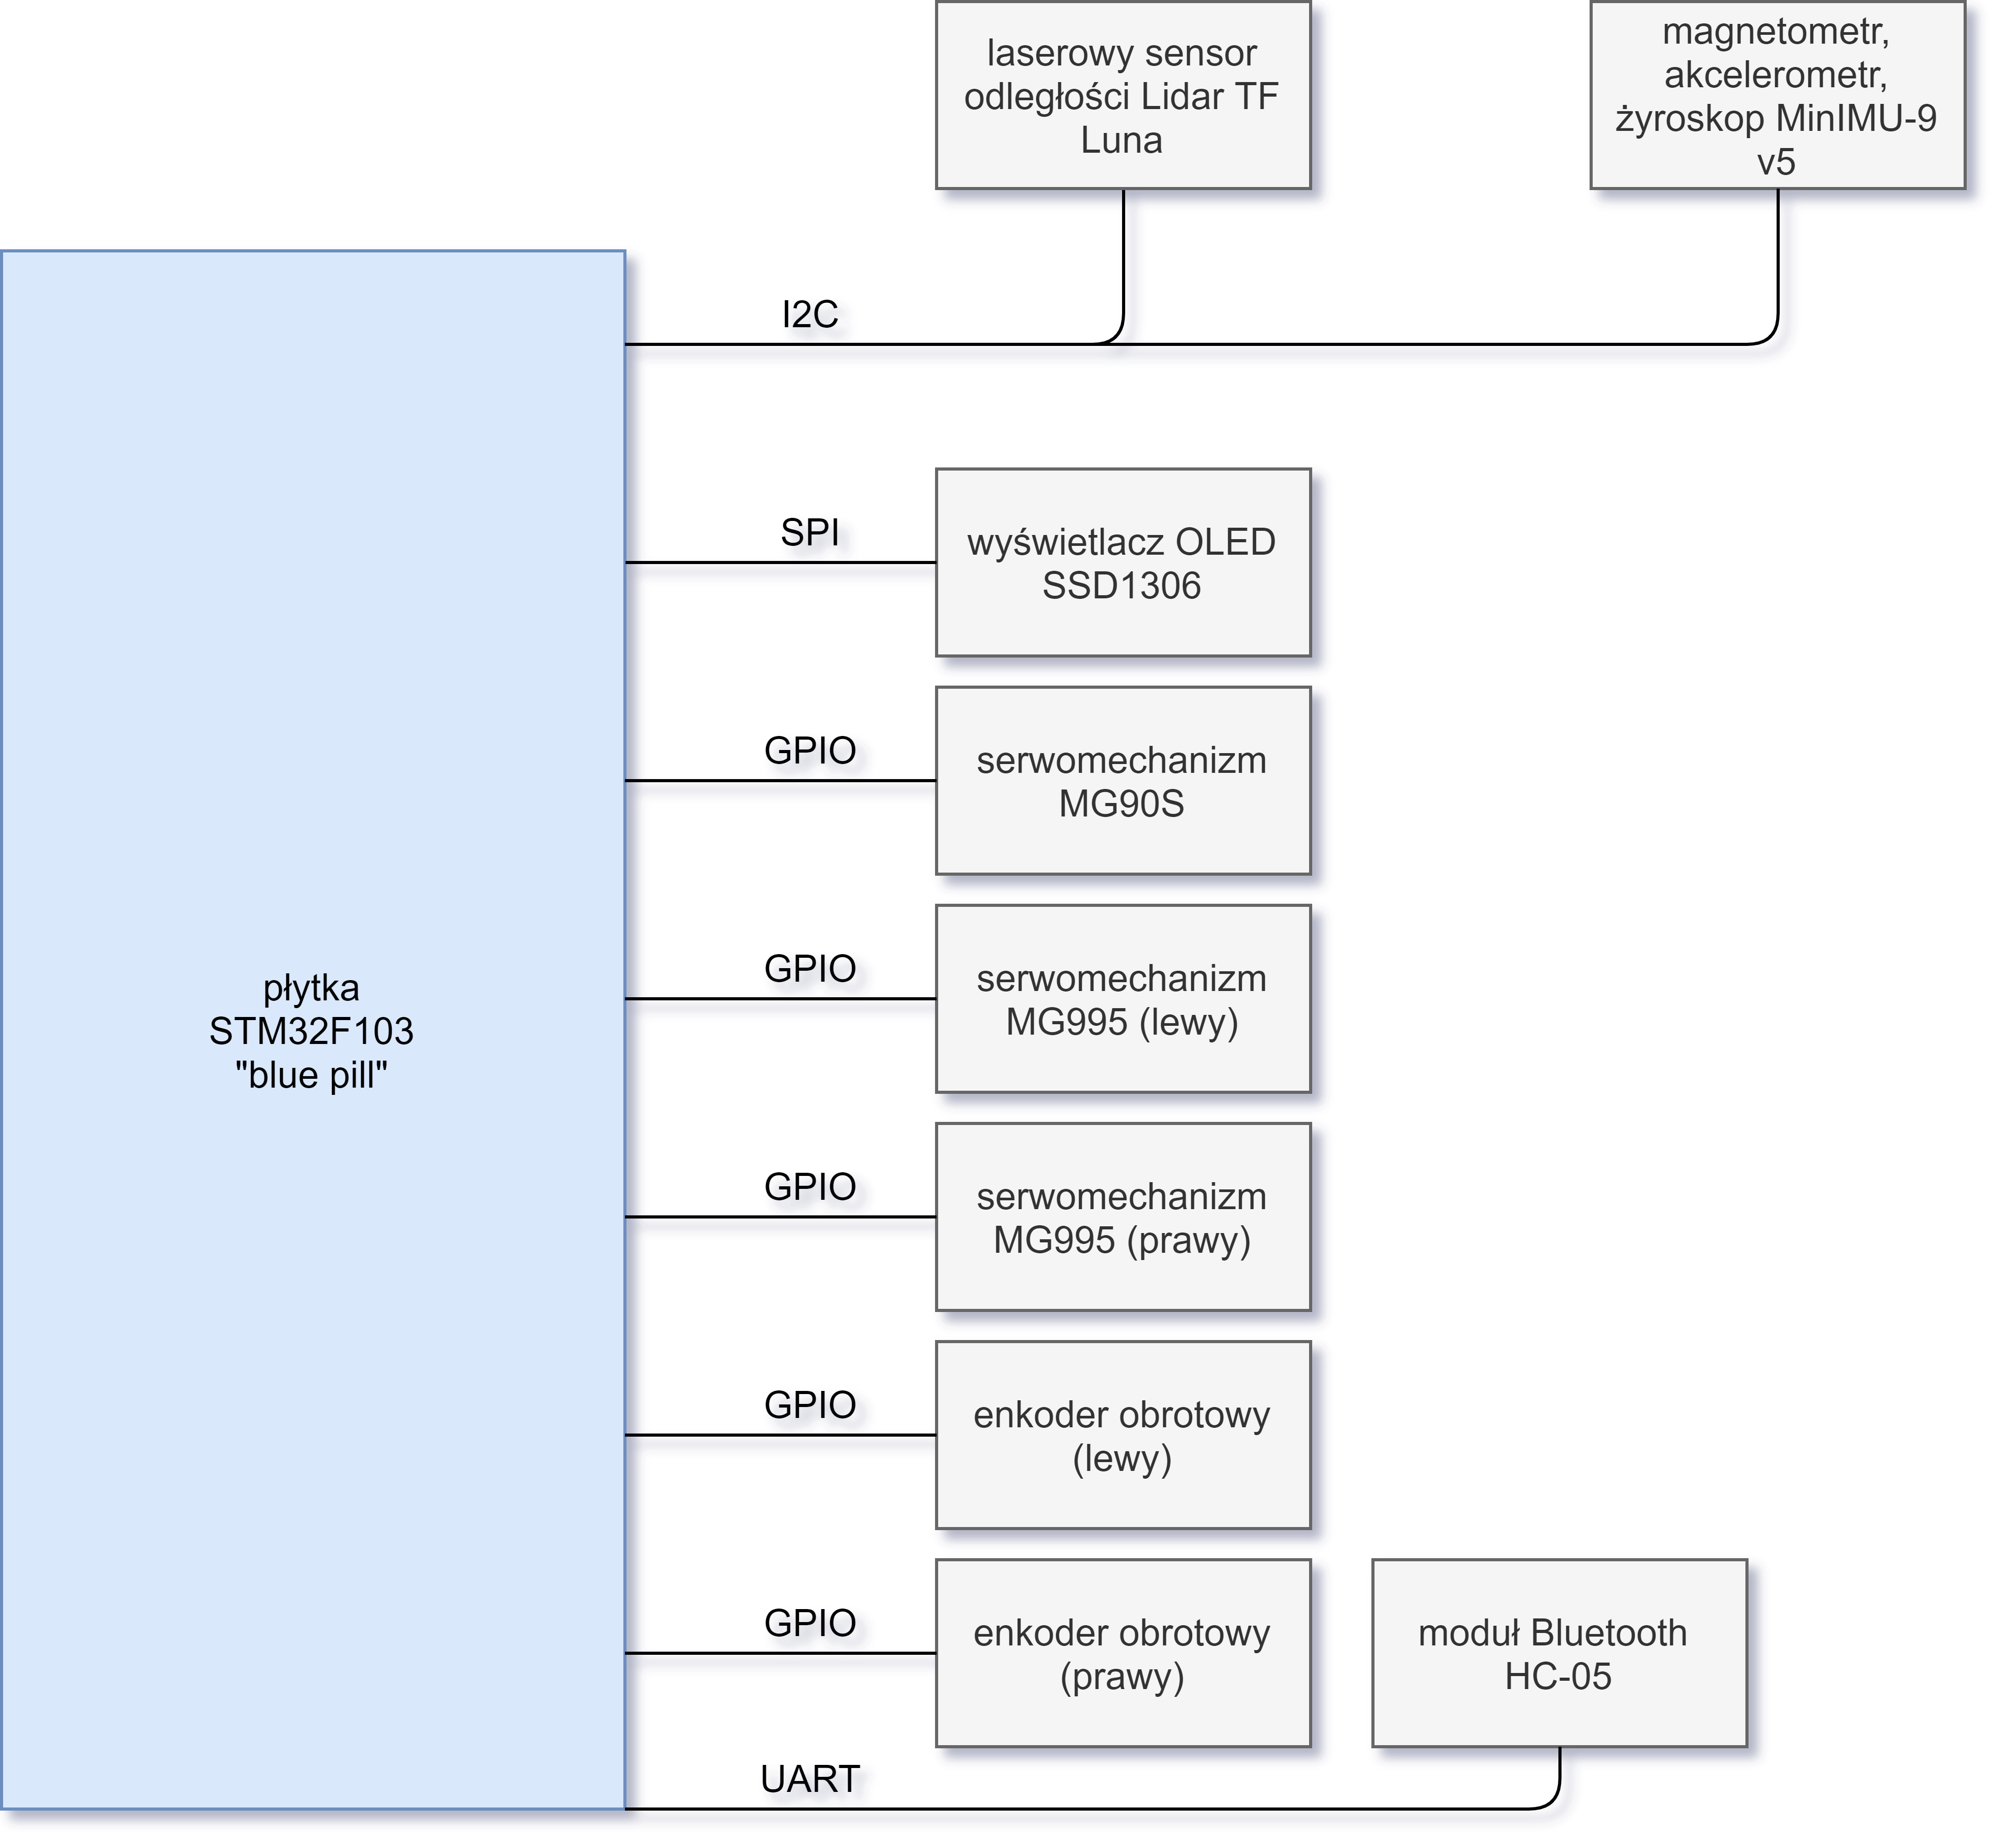
\includegraphics[width=1\linewidth]{rys/electronic-schematic.png}
	\caption{Uproszczony schemat podłączonych do jednostki sterującej peryferiów}
	\label{fig:electronic-schematic-simplified}
\end{figure}

